\documentclass[a4paper]{article}
\usepackage[utf8]{inputenc}
\usepackage[russian,english]{babel}
\usepackage[T2A]{fontenc}
\usepackage[left=10mm, top=20mm, right=18mm, bottom=15mm, footskip=10mm]{geometry}
\usepackage{indentfirst}
\usepackage{amsmath,amssymb}
\usepackage[italicdiff]{physics}
\usepackage{graphicx}
\graphicspath{{images/}}
\DeclareGraphicsExtensions{.pdf,.png,.jpg}
\usepackage{wrapfig}
\usepackage{float}
\usepackage{subcaption}
\usepackage{enumitem}
\usepackage{pdflscape}
\usepackage{caption}
\usepackage{array}

\captionsetup[figure]{name=Рисунок}
\captionsetup[table]{name=Таблица}

\title{\underline{Отчет о выполненной лабораторной работе}}
\author{Воронин Денис Б04-407}

\begin{document}

\maketitle

\begin{center}
\textbf{\Large Тепловое излучение}
\end{center}

\textbf{Цель работы:} при помощи модели АЧТ провести измерения температуры оптическим пирометром с исчезающей нитью и термопарой, исследовать излучение накаленных тел с различной испускательной способностью, определить постоянные Планка и Стефана - Больцмана.

\textbf{В работе используются:} блок питания, тумблер для переключения режимов нагрева, оптический пирометр, вольтметр и цепи термопары, модель АЧТ (керамическая трубка), трубка с кольцами с разной излучательной способностью, лампа накаливания.

\section{Аннотация}

По окончании работы должны будем измерить яркостную температуры поверхности трубки и каждого из колец, замерить яркостную температуру лампочки накаливания и по этим данным найти термодинамическую температуру вольфрамовой нити лампы, вычислить для каждого значения ТД температуры мощность, потребляемую нитью лампы. 
Построить график и проверить закон Стефана - Больцмана и найти ее величину. По найденным значениям Постоянной Больцмана найти значение постояной Планка.

\section{Теоретические сведения}

Соотношение неопределенностей Гейзенберга:
\[
\Delta x \, \Delta p_x \geqslant 2\pi\hbar. \tag{1}
\]

Число разрешенных состояний частиц N: 

\[
N = (2J + 1) \frac{\Gamma}{(2\pi\hbar)^3}. \tag{2}
\]

где фазовый объем:

\[
\Gamma = \frac{4}{3} \pi p^3 V.\tag{3}
\]

Есть два вида частиц: Ферми частицы и Бозе частицы. Ферми частицы (фермионы) имеют полуцелый спин и антисимметричную волновую функцию.
Бозе частицы (бозоны) имеют целый спин и симметричную волновую функцию.\par

Число переходов из одного состояния в другое и наоборот за большой промежуток времени будут равны
\[N_{12} = N_{21}\]

Преобразуя эту формулу можно получить число переходов из возбужденного состояния:

\[
n_{21} = \frac{N_{21}}{t_1} = n W_{12}^{(1)} + W_{12}^{(1)} = W_{\text{инд}} + W_{\text{сп}}. \tag{4}
\]

При равновесии число фотонов с частотой $\omega$:

\[
\overline{n} = \frac{1}{e^{\hbar\omega/(k_{\mathrm{B}}T)} - 1}.\tag{5}
\]

Полная испускательная способность (или энергетическая светимость):

\[
R = \frac{W}{S}.\tag{6}
\]

Спектральная испускательная способность:

\[
r_{\lambda, T} = \frac{dR}{d\lambda}.\tag{7}
\]

Спектральная поглощающая способность:

\[
a_{\lambda, T} = \frac{\Phi_{\lambda\,\text{погл}}}{\Phi_{\lambda\,\text{пад}}}.\tag{8}
\]

Коэффициент поглощения: 

\[
A(T) = \frac{\Phi_{\text{погл}}}{\Phi_{\text{пад}}}.\tag{9}
\]

Закон Кирхгофа: 

\[
\frac{r_{\lambda, T}}{a_{\lambda, T}} = f(\lambda, T).\tag{10}
\]

Закон Кирхгофа для АЧТ:

\[
r_{\lambda, T} = f(\lambda, T) = r_{\lambda, T}^{\text{ачт}}.\tag{11}
\]

Закон Кирхгофа для нечерных тел:

\[
r_{\lambda, T} = a_{\lambda, T} \, r_{\lambda, T}^{\text{ачт}}.\tag{12}
\]

Закон Стефана - Больцмана для АЧТ:

\[
R_T^{\text{ачт}} = \sigma T^4, \tag{13}
\]

Закон Стефана - Больцмана для нечерных тел:

\[
R_T^{\text{ачт}} =\epsilon \sigma T^4, \tag{14}
\]

Постоянная Стефана - Больцмана:

\[
\sigma = \frac{2\pi^5 k_{\mathrm{B}}^4}{15 c^2 h^3} = 5{,}67 \cdot 10^{-12} \; \frac{\text{Вт}}{\text{см}^2 \cdot \text{К}^4}\tag{15}
\]

Постоянная Планка:

\[
h = \sqrt[3]{\frac{2\pi^5 k_{\mathrm{B}}^4}{15 c^2 \sigma}}.\tag{16}
\]

Закон смещения Вина:

\[
\lambda_{\max} T = b = 0{,}2897 \; \text{см} \cdot \text{К}.\tag{17}
\]

\begin{figure}[!hb]
	\centering
	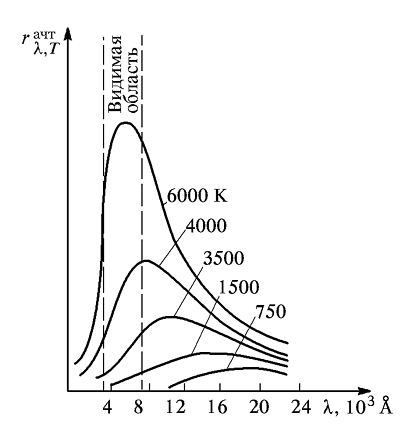
\includegraphics[width=0.35\linewidth]{p2.png}
	\caption{Распределение энергии в спектре излучения АЧТ при различных температурах.}
	\label{pic_2}
\end{figure}

Различают 3 температуры: радиационную, цветовую и яркостную.\par

Радиациооная температура - это температура АЧТ, при которой интегральная испускательная способность совпадает с интегральной испускательной способностью изучаемого тела.\par

Цветовая температура - это температура, при которой отгошение между спектральными испускательными способностями остается постоянным.\par

Яркостная температура - это температура АЧТ, при которой его спектральная испускательная способность совпадает со спектральной испускательной способность изучаемого тела.\par

Если бы нить была бы АЧТ, то мощность, протребляемая нитью была:

\[
W = \sigma S (T^4 - T_0^4),\tag{18}
\]

Но, если учесть, что оно не черное, то:

\[
W = \varepsilon_T S \sigma T^4,\tag{19}
\]

\section{Ход работы}

$\textbf{1. Опробование работы оптического пирометра}$ \par

Измерим с помощью пирометра температуру АЧТ и сравним ее со значением температуры, измеренной при помощи термопарного термометра.\par

Для этого включим и прогреем прибор и добъемя четкого изображения дна АЧТ. Далее выведим красный светофильтр пирометра и начнем проводить карлибровку для двух разных напряжений снизу вверх и потом сверху вниз (12 значений):

\begin{table}[h]
\centering
\begin{tabular}{|c|c|}
\hline
Сверху, t $^{\circ} C $ & Снизу, t $^{\circ} C $\\
\hline
964 & 930 \\
\hline
963 & 935 \\
\hline
963 & 938 \\
\hline
\end{tabular}
\caption{Напряжение 38250 мкВ }
\label{tab:example}
\end{table}

\begin{table}[h]
\centering
\begin{tabular}{|c|c|}
\hline
Сверху, t $^{\circ} C $ & Снизу, t $^{\circ} C $\\
\hline
937 & 918 \\
\hline
930 & 921 \\
\hline
936 & 920 \\
\hline
\end{tabular}
\caption{Напряжение 36830 мкВ}
\label{tab:example}
\end{table}

\begin{figure}[!hb]
	\centering
	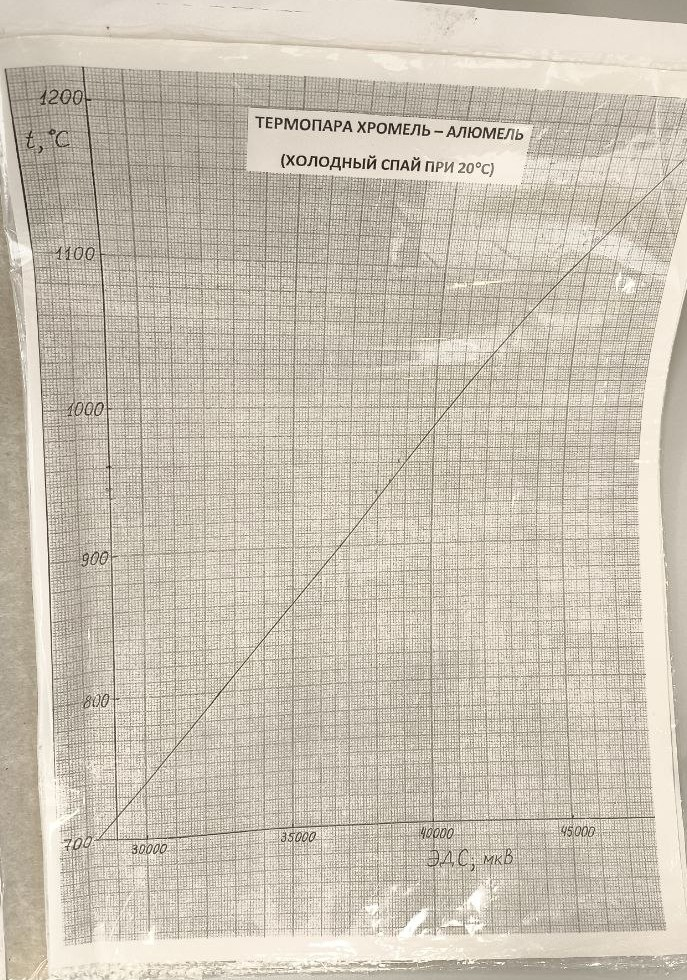
\includegraphics[width=0.3\linewidth]{Convert.jpg}
	\caption{Термопара хромель - алюмель (хододный спай при 20$^{\circ} C $)}
	\label{pic_2}
\end{figure}

\newpage

По графику определим температуру, которой соответствует напряжение в этих двух измерениях:\par

\[ 38250 \text{мкВ} = 940^{\circ} C \]

\[ 36830 \text{мкВ} = 910^{\circ} C \]

Убедились, что значения температуры, получаемые разными способами мало отличаются друг от друга (1-3$\%$)

$\textbf{2. Измерение яркостной температуры накаленных тел}$ \par

Цель показать, что тела с одинаковой тд температурой имеют разную яркостную.\par

Для этого направим пирометр на поверхность керамической трубы с кольцами из различных материалов и измерим яркостную температуру:

\begin{table}[h]
\centering
\begin{tabular}{|c|c|}
\hline
Трубка & 800 $^{\circ} C $ \\
\hline
Левое кольцо & 844 $^{\circ} C $ \\
\hline
Правое кольцо& 847 $^{\circ} C $ \\
\hline
\end{tabular}
\caption{Измерение яркостной температуры}
\label{tab:example}
\end{table}

Это объясняется тем, что яркостная температура - это температура АЧТ при которой спектральная испускательная способность АЧТ совпадает со спектральной испускательной способностью изучаемого тела. Значит эти два кольца изготовлены из разных материалов или в них используется разный сплав.

$\textbf{3. Проверка закона Стефана - Больцмана}$ \par

Направим прирометр на лампу накаливания и измерим пирометром яркостную температуру в диапозоне от 900$^{\circ} C $ до 1900$^{\circ} C $. 

\begin{table}[h]
\centering
\begin{tabular}{|c|c|c|c|c|}
\hline
T, K & I, A & V, B & $T_{\text{тд}}$, K & P, Вт \\
\hline
1173 & 0.499 & 1.55 & 1220 & 0.77 \\
\hline
1273 & 0.538 & 1.89 & 1320 & 1.02 \\
\hline
1373 & 0.586 & 2.32 & 1420 & 1.36 \\
\hline
1473 & 0.637 & 2.80 & 1520 & 1.78 \\
\hline
1573 & 0.669 & 3.12 & 1620 & 2.09 \\
\hline
1673 & 0.735 & 3.81 & 1720 & 2.80 \\
\hline
1773 & 0.799 & 4.51 & 1820 & 3.60 \\
\hline
1873 & 0.846 & 5.07 & 1920 & 4.29 \\
\hline
1973 & 0.907 & 5.81 & 2020 & 5.27 \\
\hline
2073 & 0.967 & 6.58 & 2120 & 6.36 \\
\hline
2173 & 1.045 & 7.62 & 2220 & 7.96 \\
\hline
\end{tabular}
\caption{Экспериментальные и вычисленные данные для вольфрамовой нити}
\label{tab:data_full}
\end{table}

Из графика рис 5 определили величину n = 4.012\par

Найдем величину постоянной Стефана - Больцмана по формуле для каждого значения, превышающего 1700K:

\[\sigma = \frac{P}{\varepsilon_{T}ST_\text{тд}^{4}}\]

\begin{align*}
\sigma_1 &= \frac{3{,}60}{0{,}2256 \cdot 3{,}6 \cdot 10^{-5} \cdot 1820^4} = (4{,}04 \pm 0{,}13) \cdot 10^{-8} \text{ Вт}/(\text{м}^2 \cdot \text{К}^4) \\
\sigma_2 &= \frac{4{,}29}{0{,}2386 \cdot 3{,}6 \cdot 10^{-5} \cdot 1920^4} = (3{,}68 \pm 0{,}11) \cdot 10^{-8} \text{ Вт}/(\text{м}^2 \cdot \text{К}^4) \\
\sigma_3 &= \frac{5{,}27}{0{,}2516 \cdot 3{,}6 \cdot 10^{-5} \cdot 2020^4} = (3{,}49 \pm 0{,}11) \cdot 10^{-8} \text{ Вт}/(\text{м}^2 \cdot \text{К}^4) \\
\sigma_4 &= \frac{6{,}36}{0{,}2646 \cdot 3{,}6 \cdot 10^{-5} \cdot 2120^4} = (3{,}31 \pm 0{,}10) \cdot 10^{-8} \text{ Вт}/(\text{м}^2 \cdot \text{К}^4) \\
\sigma_5 &= \frac{7{,}96}{0{,}2776 \cdot 3{,}6 \cdot 10^{-5} \cdot 2220^4} = (3{,}28 \pm 0{,}10) \cdot 10^{-8} \text{ Вт}/(\text{м}^2 \cdot \text{К}^4)
\end{align*}

\newpage

\begin{figure}[!hb]
	\centering
	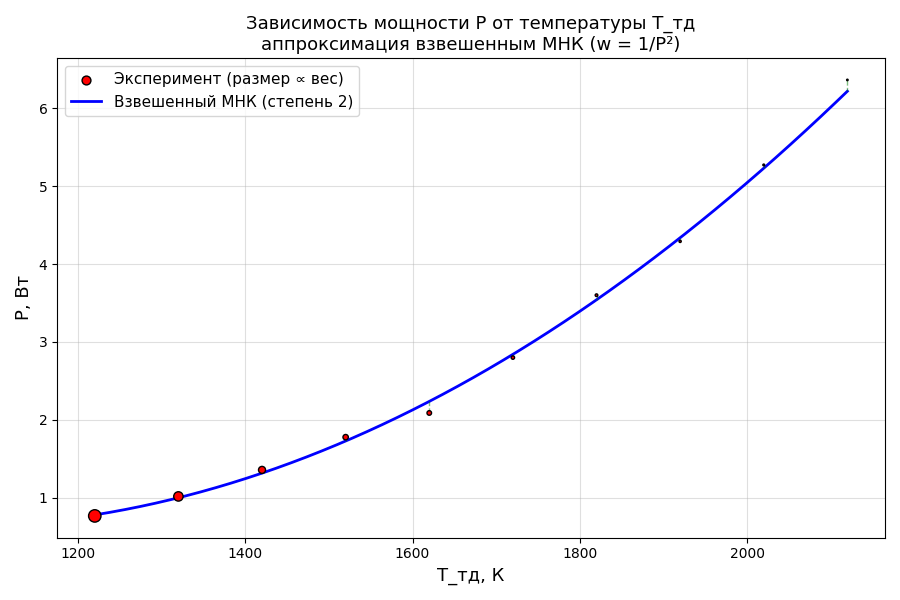
\includegraphics[width=0.7\linewidth]{F1.png}
	\caption{График зависимости P($T_\text{тд}$)}
	\label{pic_2}
\end{figure}

% Аппроксимация: P(T) = 4.796617e-06·T² + -9.985374e-03·T + 5.8261
% Взвешенная сумма квадратов остатков (χ²) = 0.0085
% Среднеквадратичное отклонение (невзвешенное) = 0.0753 Вт

Для провекри закона Стефана - Больцмана построим в логарифмическом масштабе график:

\begin{figure}[!hb]
	\centering
	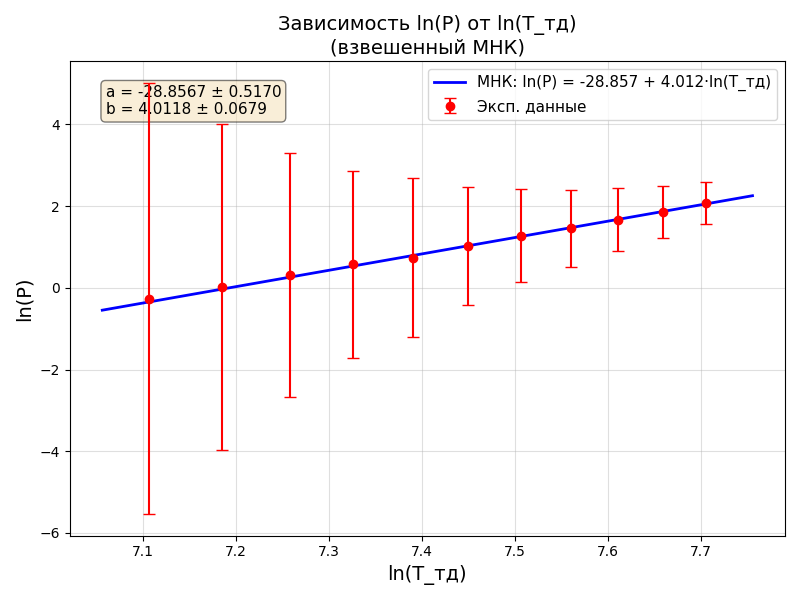
\includegraphics[width=0.7\linewidth]{F2.png}
	\caption{График зависимости ln(P)ln($T_\text{тд}$)}
	\label{pic_2}
\end{figure}

Вычислим постоянную Планка по формуле:

\[
h = \sqrt[3]{\frac{2\pi^5 k_{\mathrm{B}}^4}{15 c^2 \sigma}}.
\]

\begin{align*}
h_1 &= \sqrt[3]{\frac{2\pi^5 \cdot (1{,}38 \cdot 10^{-23})^4}{15 \cdot (3 \cdot 10^8)^2 \cdot 4{,}04 \cdot 10^{-8}}} = (7{,}42 \pm 0{,}08) \cdot 10^{-34} \text{ Дж} \cdot \text{с} \\
h_2 &= \sqrt[3]{\frac{2\pi^5 \cdot (1{,}38 \cdot 10^{-23})^4}{15 \cdot (3 \cdot 10^8)^2 \cdot 3{,}68 \cdot 10^{-8}}} = (7{,}66 \pm 0{,}08) \cdot 10^{-34} \text{ Дж} \cdot \text{с} \\
h_3 &= \sqrt[3]{\frac{2\pi^5 \cdot (1{,}38 \cdot 10^{-23})^4}{15 \cdot (3 \cdot 10^8)^2 \cdot 3{,}49 \cdot 10^{-8}}} = (7{,}79 \pm 0{,}08) \cdot 10^{-34} \text{ Дж} \cdot \text{с} \\
h_4 &= \sqrt[3]{\frac{2\pi^5 \cdot (1{,}38 \cdot 10^{-23})^4}{15 \cdot (3 \cdot 10^8)^2 \cdot 3{,}31 \cdot 10^{-8}}} = (7{,}93 \pm 0{,}08) \cdot 10^{-34} \text{ Дж} \cdot \text{с} \\
h_5 &= \sqrt[3]{\frac{2\pi^5 \cdot (1{,}38 \cdot 10^{-23})^4}{15 \cdot (3 \cdot 10^8)^2 \cdot 3{,}28 \cdot 10^{-8}}} = (7{,}96 \pm 0{,}08) \cdot 10^{-34} \text{ Дж} \cdot \text{с}
\end{align*}

$\textbf{4. Измерение яркостной температуры неоновой лампочки}$ \par

Яркостная температура неоновой лампочки составила: 827$^{\circ} C $ \par

Это можно объяснить тем, что спектральная испускательная способность неоновой лампочки самая близкая к спектральной испкскательной спобности АЧТ.

\section{Вывод}

При помощи модели АЧТ провели измерения температуры оптическим пирометром, исследовали излучение накаленных тел с различной испкскательной способностью и рассчитали постоянные Планка и Стефана - Больцмана.

\end{document}